%\documentclass[c,handout]{beamer}
\documentclass[c,xcolor=table]{beamer}


\usepackage{etex}
\usepackage{advdate}
\usetheme{Unicam}


\title{Applying Process Mining in Blockchain Transactions}

\author{Massimiliano Sampaolo}

%\usetheme{lucid}
\begin{document}
	
\SetDate[30/01/2019]

	\frame {
		\titlepage
		Supervisor: Barbara Re\\
		Second supervisor: Andrea Morichetta
    }
	
	
	\frame {
		\frametitle{Objective and Motivations}
		The thesis want to understand and define bindings between \textbf{blockchain} transactions 
		using \textbf{process mining}\\ \vspace{20px}
		Why?
		\begin{itemize}
			\item Blockchain and process mining are hot topics in industry and academia
			\item Infer and analyse the behaviour of systems to increase their quality
			\item Give a graphical representation of processes defined by software systems
		\end{itemize}
	}
	
    
	\frame{
		\frametitle{Blockchain}

		\begin{figure}[T]
			\centering
			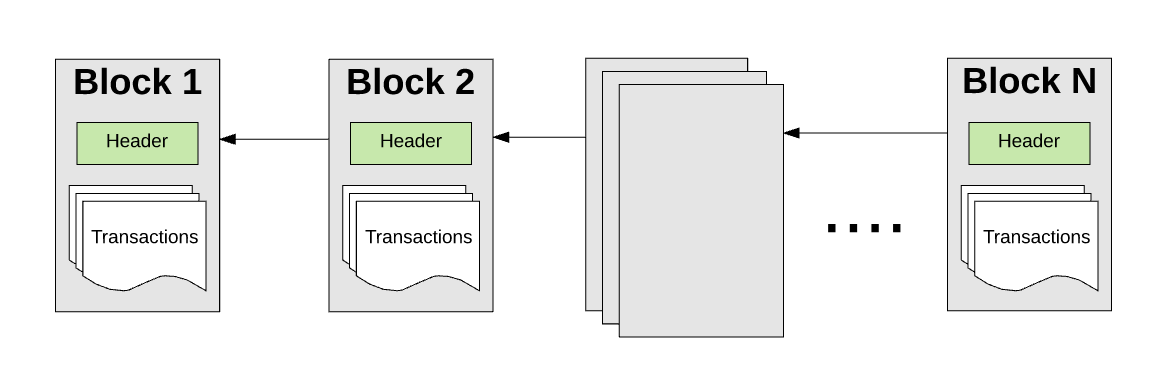
\includegraphics[width=70mm]{images/chain_of_blocks.png}
		\end{figure}

		Blockchain characteristics:
		\begin{itemize}
			\item Decentralization
			\item Trasparency
			\item Security
			\item Immutability
		\end{itemize}

		\vspace{8px}

		\textbf{Ethereum}: Vritual machine, Smart contracts and decentralized applications
    }
	
	
	\frame{
	    \frametitle{Business Process and Process Mining}
		
		\textbf{Business Process} is a collection of related and structured activities undertaken by one or more 
		organisations in order to pursue some particular goal

		\vspace{16px}
		
		Process mining has the goal to discover, monitor and improve real processes by extracting knowledge from event logs 
		readily available in today's information systems

		\vspace{16px}

		Three form of process mining:
		\begin{itemize}
			\item Process discovery
			\item Conformance checking
			\item Enhancement
        \end{itemize}
        
        Discovery algorithms: Heuristic Miner, Inductive Miner, Split Miner
	}
	
	\frame{
		\frametitle{Methodology}

		\begin{figure}[t]
			\centering
			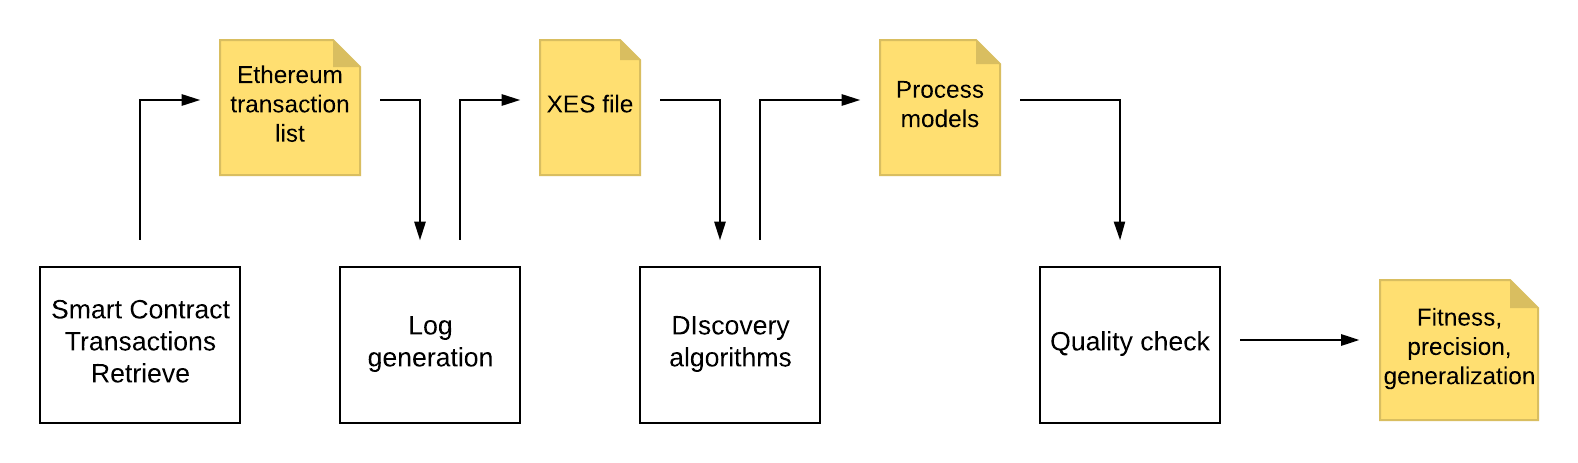
\includegraphics[width=120mm]{images/methodology.png}
		\end{figure}
    }
    
    \frame {
        \frametitle{Case studies}

        \begin{itemize}
            \item \textbf{RoToHive}, a new type of fantasy sports site that runs weekly tournaments
            \item \textbf{Fomo 3D}, lottery game in which the last person to buy a key at the end of a round wins the jackpot
            \item \textbf{IDEX}, cryptocurrency exchange that allows the user to deposit, withdraw or exchange cryptocurrencies
        \end{itemize}
    }

	\frame{
		\frametitle{RoToHive}

		\begin{figure}[t]
			\centering
			
\includegraphics[width=40mm]{images/rotohive.png}
		\end{figure}

		RotoHive is a new type of fantasy sports site that runs weekly tournaments
		
		Model discovered with Heuristic Miner:

		\begin{figure}
			\centering
			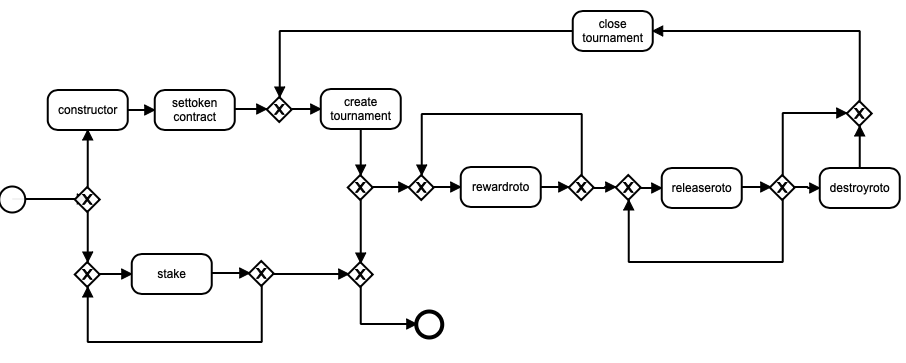
\includegraphics[width=90mm]{images/roto_heuristic.png}
		\end{figure}
    }
    

	\frame{
		\frametitle{Supporting tool}
		
		The system designed recreates the methodology used in the case studies analysis.

		\vspace{16px}

		The architecture of the Mining Framework: 

		\begin{figure}[t]
			\centering
			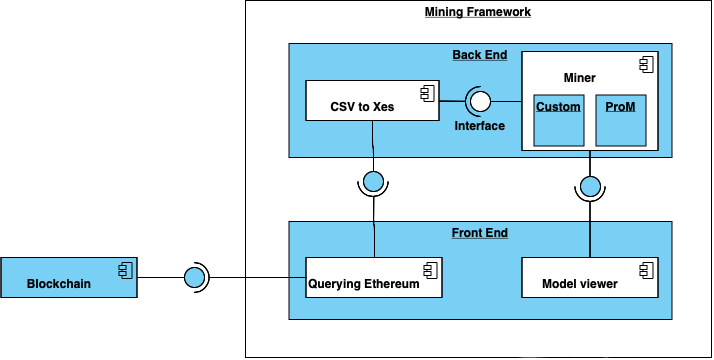
\includegraphics[width=80mm]{images/component_diagram.png}
		\end{figure}
	}


	\frame{
		\frametitle{Conclusion and Lessons learned}

		Sound models discovered and pretty good quality parameters measured

		\vspace{16px}

		The three algorithms obtained similiar results. How well an algorithm fits a specific application domain depends from 
		the domain itself regardless the fact that it uses the Blockchain

		\vspace{16px}

		The analysis infer the logic of the system and can be used to increase solution quality, or understand how users interact with 
		a product.
	}


	\frame {
		\begin{center}
			{\huge Thanks for your attention!}
		\end{center}
	}
    
\end{document}